\section{Versuchsaufbau}

Das Mach-Zehnder-Interferometer wurde mit Hilfe des Mikro-Bank-Systems Linos aufgebaut. Es bestand aus zwei Strahlteilerwürfeln und zwei um $45\degre$ angewinkelten Planspiegeln (siehe Abbildung~\ref{fig:skizze}). Als Lichtquelle diente ein Halbleiterlaser mit einer Wellenlänge von $\SI{532}{\nano\meter}$ und einer Leistung von $\SI{1}{\milli\watt}$ verwendet.

\begin{figure}[h!]
	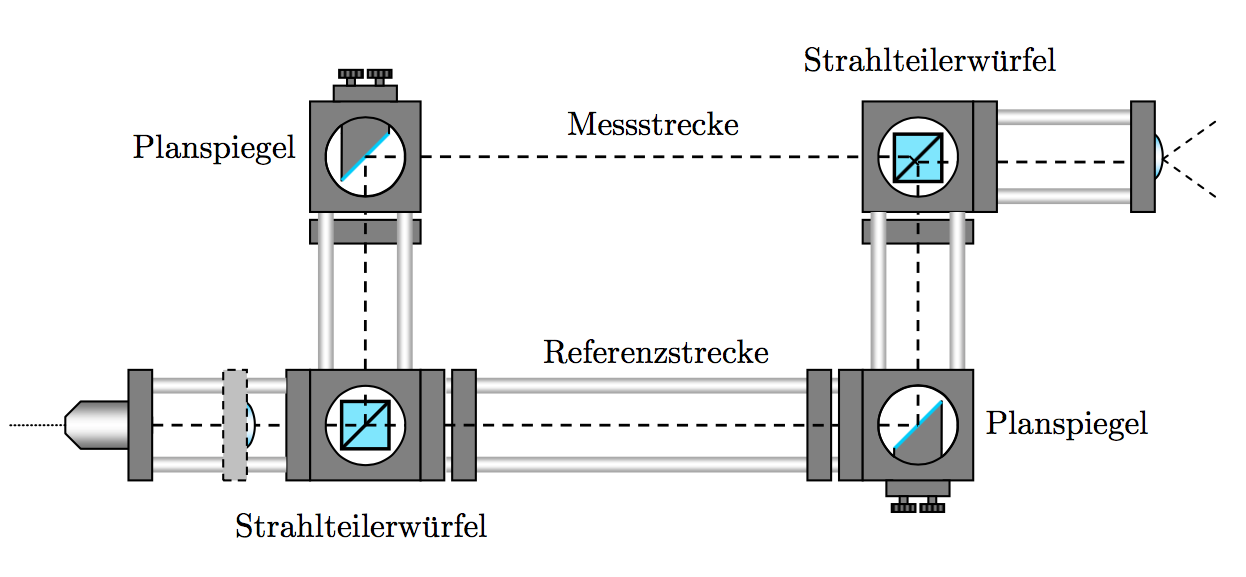
\includegraphics[width=\linewidth]{img/skizze_mzinterferometer.png}
	\caption{Prinzip - Mach-Zehnder-Interferometer}
	\label{fig:skizze}	
\end{figure}

\begin{figure}[h!]
	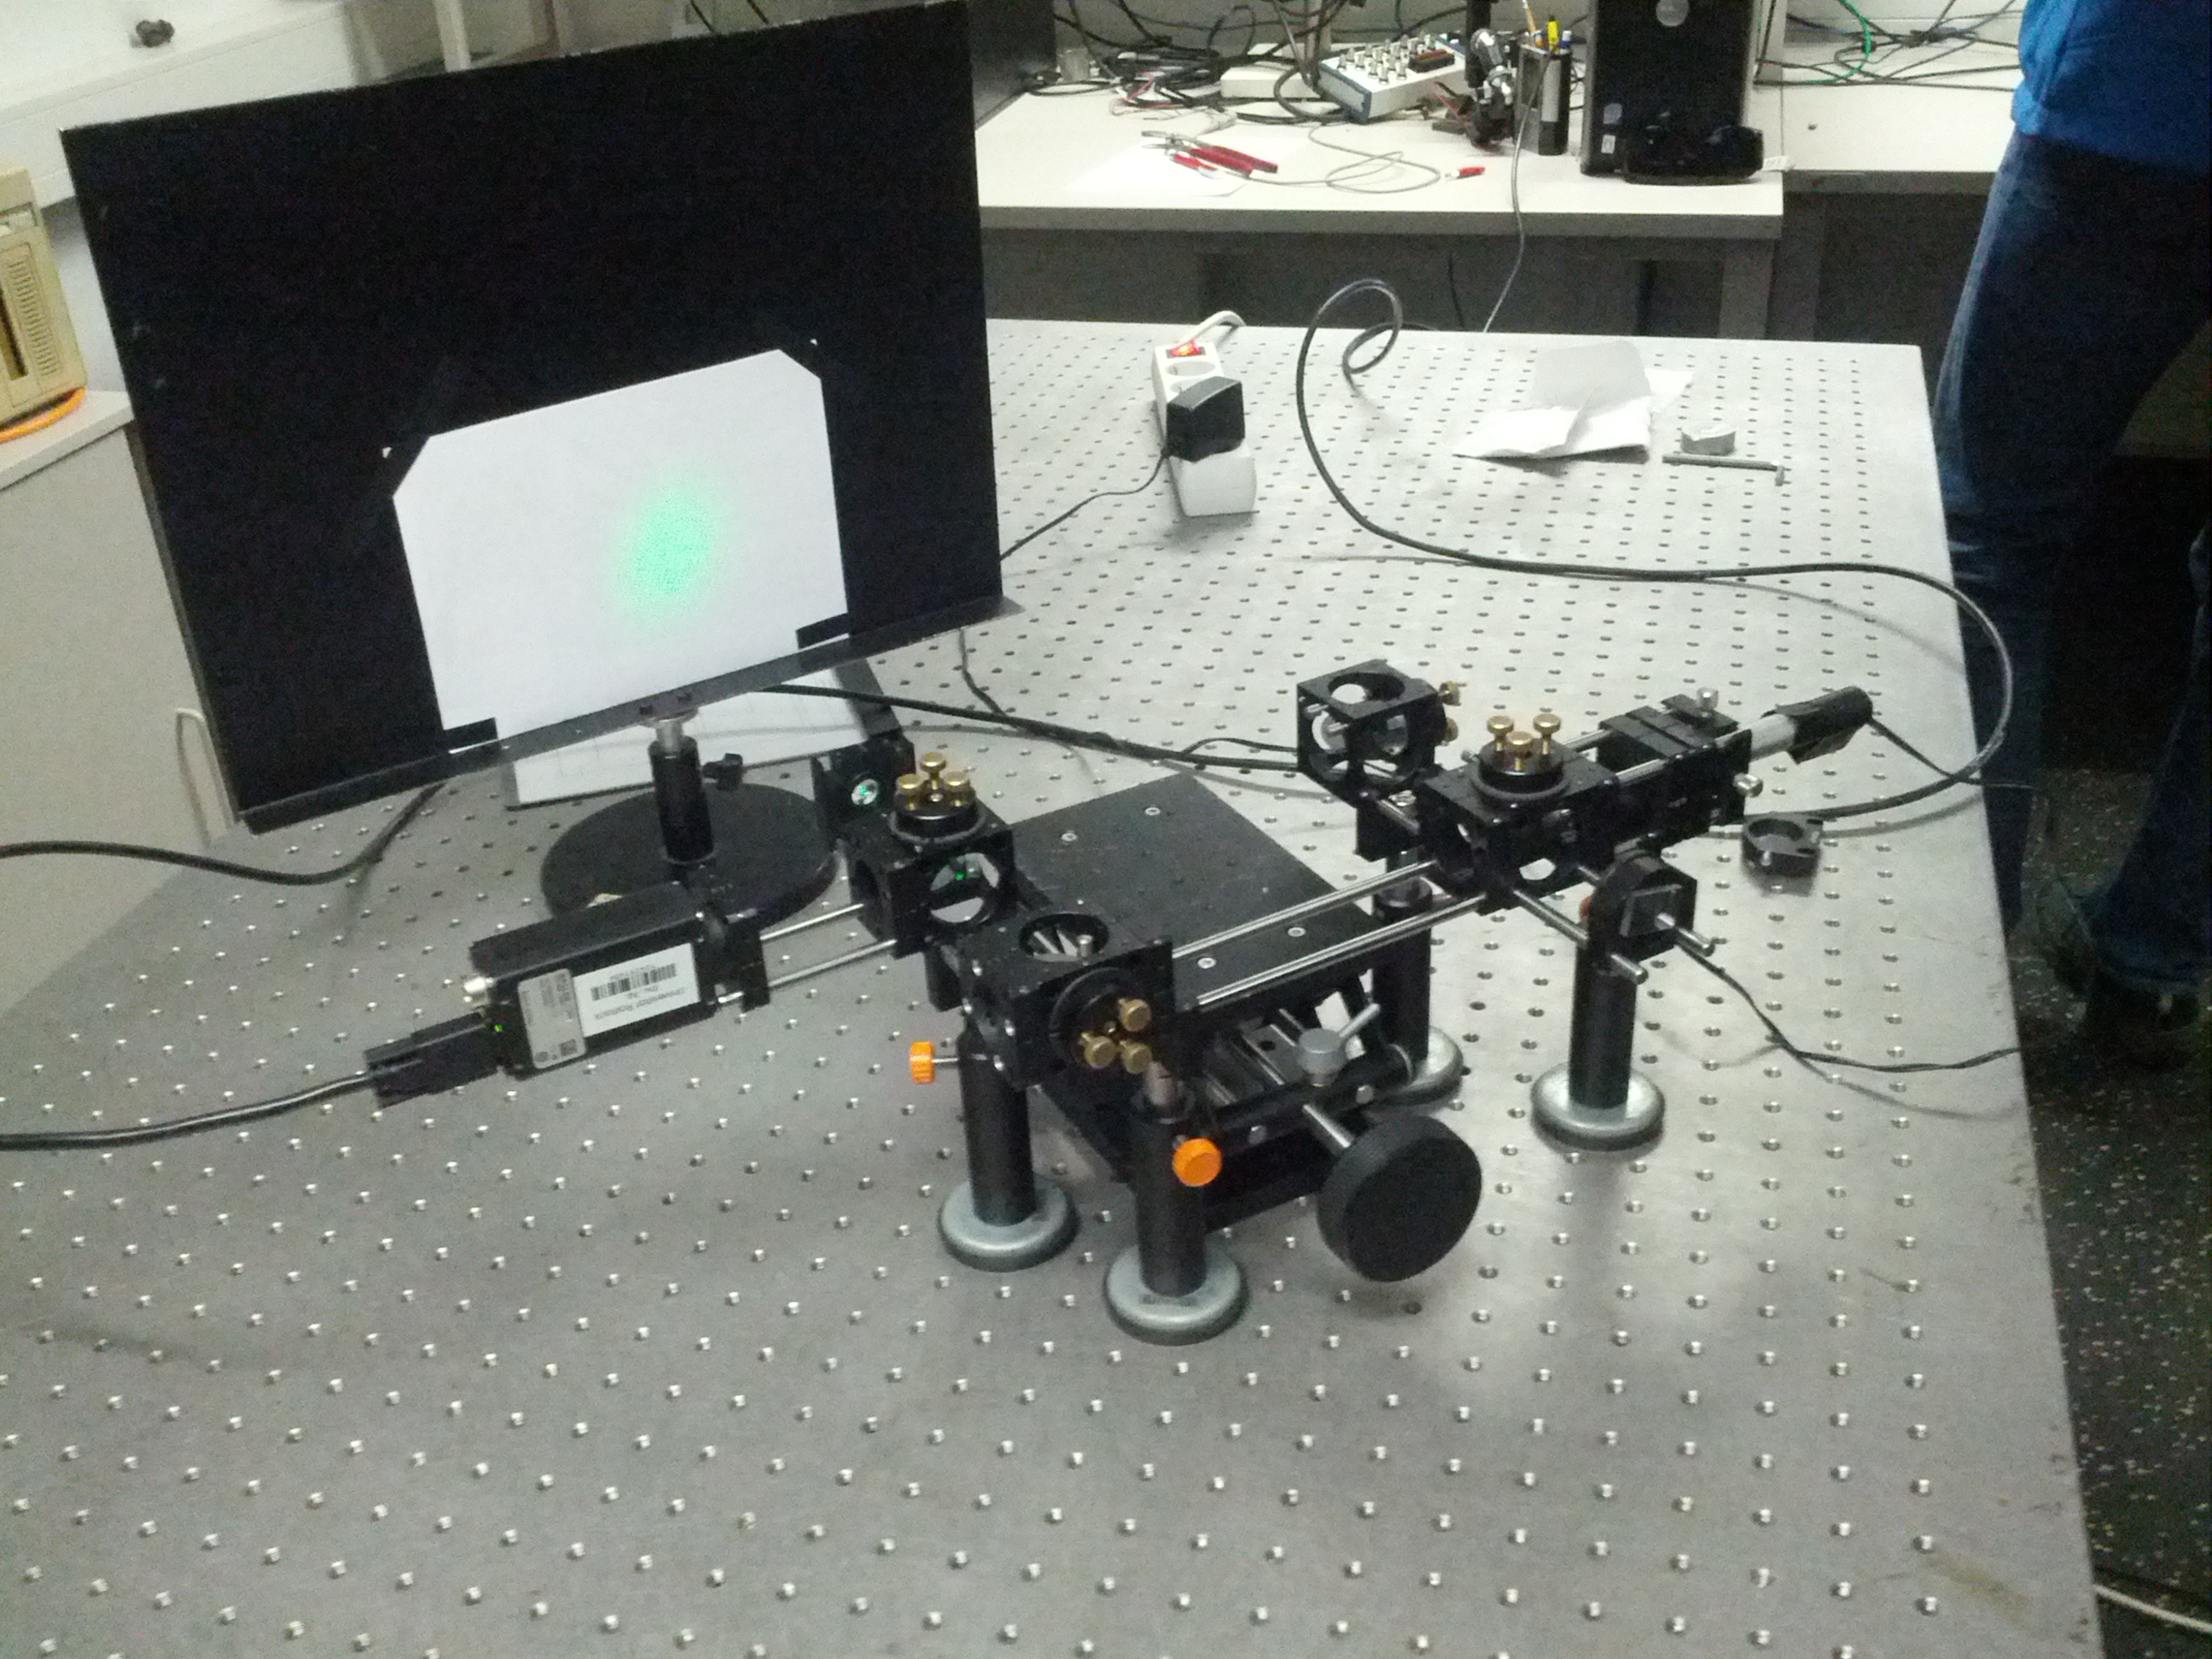
\includegraphics[width=\linewidth]{img/interferometer_aufbau}
	\caption{Versuchsaufbau - Mach-Zehnder-Interferometer}
	\label{fig:aufbau}	
\end{figure}

Um das Interferenzmuster elektronisch erfassen zu können wurde eine Kamera in einen der beiden Ausgangsstrahlen des hinteren Strahlteilerwürfels gesetzt. Zur Veranschaulichung wurde ebenfalls eine Linse im Weg des zweiten Ausgangsstrahls platziert, um das Interferenzmuster auf einem Schirm abbilden zu können (siehe Abbildung~\ref{fig:aufbau}).

Die genaue Positionierung der Strahlen erfolgte in jedem Strahlenpfad durch temporäres Einsetzten eines Pinholes und feiner Justage der optischen Komponenten. Die Strahlen wurden also alle auf dieselbe Höhe eingestellt und in der Mitte der Strecken im Mikro-Bank-System positioniert.

Für die Messung der Dickenänderung musste zunächst für jeden Durchlauf ein Referenzbild ohne ein Objekt in der Messstrecke aufgenommen werden. Dabei wurde die Belichtungszeit der Kamera so eingestellt, dass die maximale Helligkeit möglichst genau auf ein Interferenzmaximum fällt. So wurde eine Überbelichtung vermieden und die Helligkeitsauflösung maximiert. Anschließend wurde ein weiteres Bild aufgenommen, dass die Änderung des Interferenzmusters durch ein Objekt im Messpfad zeigte. 

Die Auswertung der Messung erfolgte in MathCad. Für die Berechnung musste eine einzelne geeignete Pixelzeile oder -spalten innerhalb der Bilder ausgewählt werden. Diese Messungen erfolgten für eine herkömmliche Brille, eine Laserschutzbrille und eine Linse.

Zur Veranschaulichung des praktischen Einsatzes eines Mach-Zehnder-Interferomters im Bereich der Temperaturmessung wurde am Ende noch eine Kerze in der Messstrecke positioniert.